% !TEX root = ../../thesis.tex

% \cleartoleftpage
% \includepdf{../media/chapter_illustration/poppy_prairie_2.pdf}

\chapter{Introduction} % (fold)


In the Inria Flowers team\footnote{\url{flowers.inria.fr}}, we are interested in the study of mechanisms that can allow robots and humans to autonomously and cumulatively acquire repertoires of new skills over extended periods of time.

This includes mechanisms for learning by self-exploration, as well as learning through interaction with peers, for the acquisition of both sensorimotor skills (e.g. locomotion, affordance learning and active manipulation) and social skills (e.g. grounded language use and understanding, adaptive interaction protocols, and human-robot collaboration).

An interesting evolution over the last decades has been the demonstration of the importance of robot morphology for sensorimotor control, cognition and development (\cite{kaplan2008corps} \cite{steels1995artificial} \cite{Pfeifer06}). Indeed, robot behaviour cannot be preprogramed. The actual behaviour is always emerging from a complex interaction between the control algorithm, the robot’s morphology and the environment~\cite{Steels1991emergence}. Moreover, it is clear that a well-adapted robot morphology using specific properties can greatly reduce the complexity of a given task by ensuring implicitly a part -or the entirety- of the control required~\cite{pfeifer2005morphological}.
Finally, as Rodney Brooks argued, \emph{the world is its own best model}~\cite{brooks1991intelligence} and simulators cannot realistically handle the complexity of real physics with multi-point contacts, soft material compliance, friction or unpredicted multi-modal interactions.


Exploring mechanisms of acquisition requires us to wholeheartedly focus on robot morphology.
Therefore, we \textbf{should consider robot morphology\footnote{ robot morphology is defined as any characteristic which defines the physical structure of the robot such as link sizes, number of links, joint characteristics, mass distribution, actuator characteristics, material properties, sensor characteristics and sensor placements~\cite{paul2006morphological}} as an experimental variable~\cite{kaplan2008corps} that can be tuned, and conduct experiments in the real world}.

While it is straightforward to explore and experiment with the variation of certain software parameters (e.g. algorithms, simulator), experimenting with morphological variables on a real robot is much more challenging:

\begin{enumerate}
    \item how can we have an experimental robotic platform that allows for morphology to be easily and quickly changed  while acting robustly in the real world?
    \item how can we make this project, mainly the hardware, diffusible and reusable in the research community?
\end{enumerate}

Unfortunately current robotic platforms are not suitable for addressing such challenges.

On one hand, commercial robots such as Nao \cite{gouaillier2008nao}, Darwin Op \cite{ha2011development}, Nimbro Op \cite{schwarznimbro} or iCub \cite{metta2008icub} are easily accessible and easy to use. Yet they provide a "traditional" morphology (e.g. limited compliance, rigid torso, large feet, over actuation) and modifying their morphology is impractical or impossible. Moreover in most case, they are not open source and/or the hardware is to complicated/expensive to modify.

On the other hand, lab prototypes are mainly handcrafted and specifically tuned which make them almost impossible to reproduce in another lab.

The main issue of these robots is the approaches and technologies chosen to design and produce them. Indeed, the classic way of designing and producing robots is a complicated, time-consuming and expensive process involving specific upfront tooling and complex manufacturing processes.


Within this context we decided to create a whole new humanoid robot called Poppy. This humanoid robot was designed to conduct scientific experiments easily and quickly on sensorimotor learning, exploring morphological properties, and human-robot interaction. As an experimental robotic platform, Poppy was designed to be \textbf{affordable}, \textbf{lightweight}, \textbf{robust and safe}, \textbf{easy to use}, \textbf{highly-hackable} and \textbf{fast and easy to duplicate or modify} with the goal of being easily reproducible and used by other labs thanks to an open source distribution (hardware and software). This was achieved thanks to 3D printing techniques, affordable off-the-shelf components and an optimized modular design.


% \section*{Proceeding of this thesis} % (fold)


% This thesis will be presented in 4 parts.

% In the first part, we will present related work on the role of morphology.

% The related work will be composed of 3 chapters covering important aspects associated with the Poppy project. First, we will discuss important research work on robot morphology that shows how essential robot morphology is toward

% ...
% \newpage
% \thispagestyle{empty}
% \mbox{}
% \newpage

\section{Introduction de la partie Poppy} % (fold)

Research in humanoid robotics has been thriving in recent years~\cite{hirai1998development} \cite{kaneko2008humanoid}, both due to their predicted relevance as personal and assistive robotics~\cite{tapus2007socially} \cite{oztop2005human}, and because of the scientific challenges raised by robotics with regards to cognition~\cite{asada2001cognitive}, natural communication~\cite{stiefelhagen2004natural} \cite{breazeal2002robots}, bipedal locomotion~\cite{yamaguchi1999development} \cite{chestnutt2005footstep} \cite{collins2005bipedal} and full-body physical interaction with the environment~\cite{ude2004programming}.

In the same way as the LHC is an experimental platform for exploring quantum mechanics and the origin of our universe, humanoids can act as simplified and controllable human simulators. Thus humanoid robots can be amazing tools for studying human beings and eventually contribute  to a better understanding of human behavior and abilities~\cite{atkeson2000using} \cite{cheng2007cb} \cite{brooks1986achieving}.

A famous example of such uses of humanoids was the Cog project~\cite{brooks1999cog} at the Humanoid Robotics Group of the Massachusetts Institute of Technology. This research project had two goals: an engineering goal of building a prototype general-purpose flexible and dextrous autonomous robot and a scientific goal of understanding human cognition~\cite{brooks1994building}. In particular, this project concentrated on embodiment and interaction intelligence with four aspects of a novel methodology: developmental structure, physical embodiment, integration of multiple sensory and motor systems, and social interaction. For this purpose they built several robotic platform such as a humanoid~\cite{brooks1999cog} (see \figurename~\ref{fig:brooks_and_cog}), and a very expressive multi-articulated head named Kismet~\cite{breazeal2003emotion} (see \figurename~\ref{fig:breazeal_kismet}).

% This project ended in 2003 and has brought great scientific contributions such as ... REF


\begin{figure}[t]
\centering
    \subfloat[][Rodney Brooks and the Cog humanoid]{\label{fig:brooks_and_cog}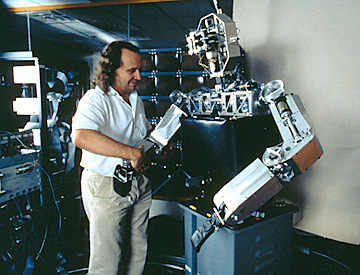
\includegraphics[height=5cm]{brooks_and_cog.jpg}}
    \hfil
    \subfloat[][Cynthia Breazeal with Kismet]{\label{fig:breazeal_kismet}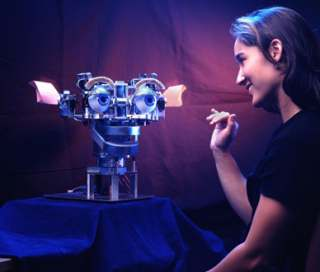
\includegraphics[height=5cm]{breazeal_kismet.jpg}}
    \caption{The Cog project was about the use of computer and robotic technology to better understand and emulate human intelligence.}
    \label{fig:cog_project}
\end{figure}



The context of this PhD thesis is grounded in the same scientific motivations as the work of R. Brooks, R. Pfeifer, T. McGeer and initiative such as the Cog project i.e. exploring the role of morphology, cognition and embodiment intelligence in several ways using real experimental robotic platforms.

The scientific approach of the Cog robots is oriented toward the exploration of embodiment in several ways, from the low level mechatronics to head design for social interactions, but robots were built 15 years ago and using classic manufacturing techniques (see \figurename~\ref{fig:cog_project}) that made them expensive, complicated to modify and especially difficult to diffuse in other laboratories.
We are now in 2014, the makers revolution is in progress~\cite{anderson} and novel technologies allow a rethink of the way we design robotic platforms, especially humanoid ones.

In the previous chapter we presented a methodology to design a robotic platform that allows both a free exploration of morphological variation and the diffusion in the research community. This method uses 3D printing to produce mechanical parts, Arduino architecture for the electronic system and python-based API for the control.

We think this design methodology can contribute to  1) the construction of better experimental robots while making the modification of robot morphology both easy and low cost, and 2) the transfer and reuse of scientific work in other laboratories through the use of open source diffusion.
Within this context we have built a whole new humanoid robot called Poppy\texttrademark (see Fig.~\ref{fig:poppy_with_me}).

\begin{figure}[tb]
    \begin{center}
        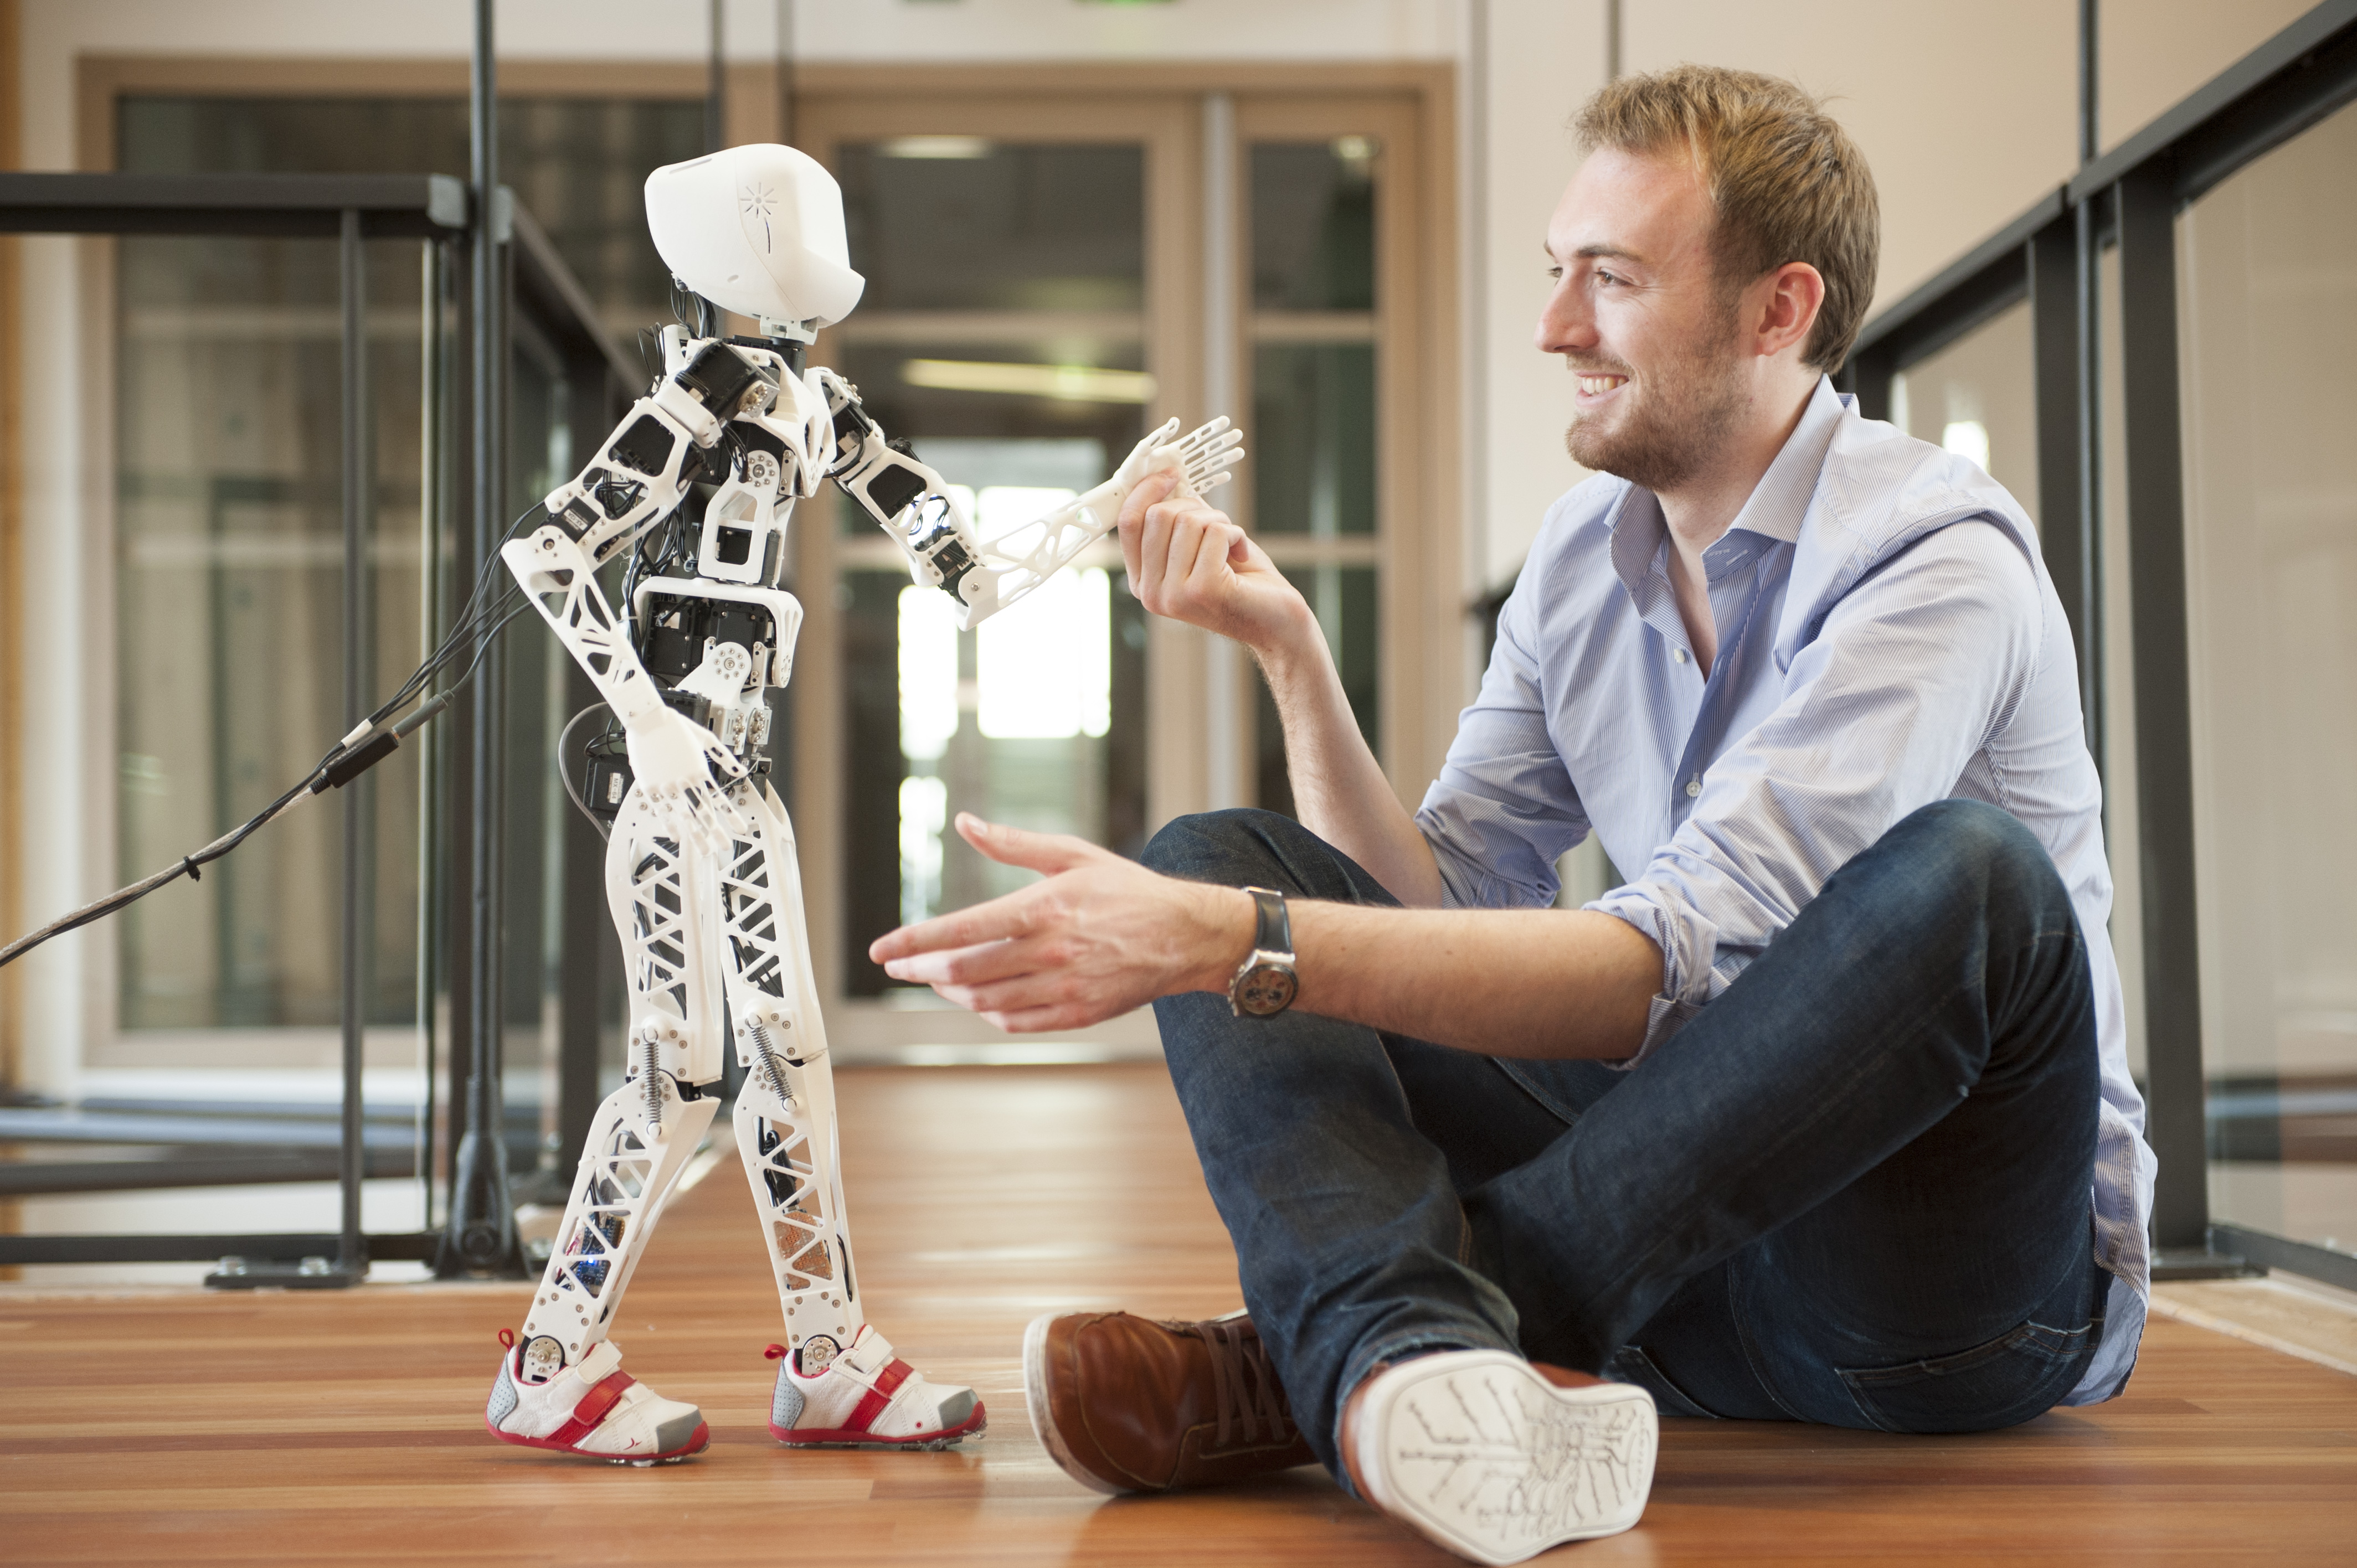
\includegraphics[width=0.7\linewidth]{lapeyre_and_poppy.jpg}
    \end{center}
    \caption{Poppy}
    \label{fig:poppy_with_me}
\end{figure}

This humanoid robot is designed to easily and quickly conduct scientific experiments on sensorimotor learning, exploring morphological properties, and human-robot interaction. As an experimental robotic platform, Poppy is designed to be \textbf{affordable}, \textbf{lightweight}, \textbf{robust and safe}, \textbf{easy to use}, \textbf{highly-hackable} and \textbf{fast and easy to duplicate or modify} with the goal to be easily reproducible and used by other labs thanks to an open source distribution (hardware and software) and the setup of modern online collaborative tools.


In this chapter, we will describe our motivation, the design guidelines we have followed and the details of Poppy's mechanical design. We will describe in more detail the open collaboration associated with the Poppy project in the chapter REF.


\section{Creating a novel humanoid robot} % (fold)

\subsection{Motivations} % (fold)

In 2012, when we started this project, none of the existing humanoid platforms were suitable for exploring the role of morphology. There were two kinds of platform. On one hand commercial robots that are rather easy to use and accessible but with a static and frozen morphology. On the other hand, prototype robots produced in labs to address specific experimentation needs, studying interesting morphologies but complicated to use and impossible to reproduce outside the lab. In both cases, only a few are open source, limiting hacks, extensions or modifications of their morphologies even further.

In the Flowers Lab, we had both kinds of robot. We used Nao (see \figurename~\ref{fig:nao_platform}) to study human robot interaction (REF PIERRE cadeau). It was really convenient for use by researchers who are not interested in hardware issue since they are addressing more high-level research challenges. Yet such a platform is limited as it is not possible to modify the robot if it is not strictly adapted to our experiment. For example, back at this time the Nao camera was not efficient, with a closed field of view and a slow framerate. We have difficultly achieved 5 frames/seconds. Although we had the necessary skills to hack Nao and change the camera to fit our needs, its hardware is not designed to be changed. Improving the vision performance would only be possible with the addition of an external camera on the Nao head which would ruin the user experience. In addition, it would have been interesting to explore how the camera parameters (FOV, framerate, resolution...) can change the user experience but again, it is not possible with this robot.

\begin{figure}[]
\centering
    \subfloat[][Nao]{\label{fig:nao_platform}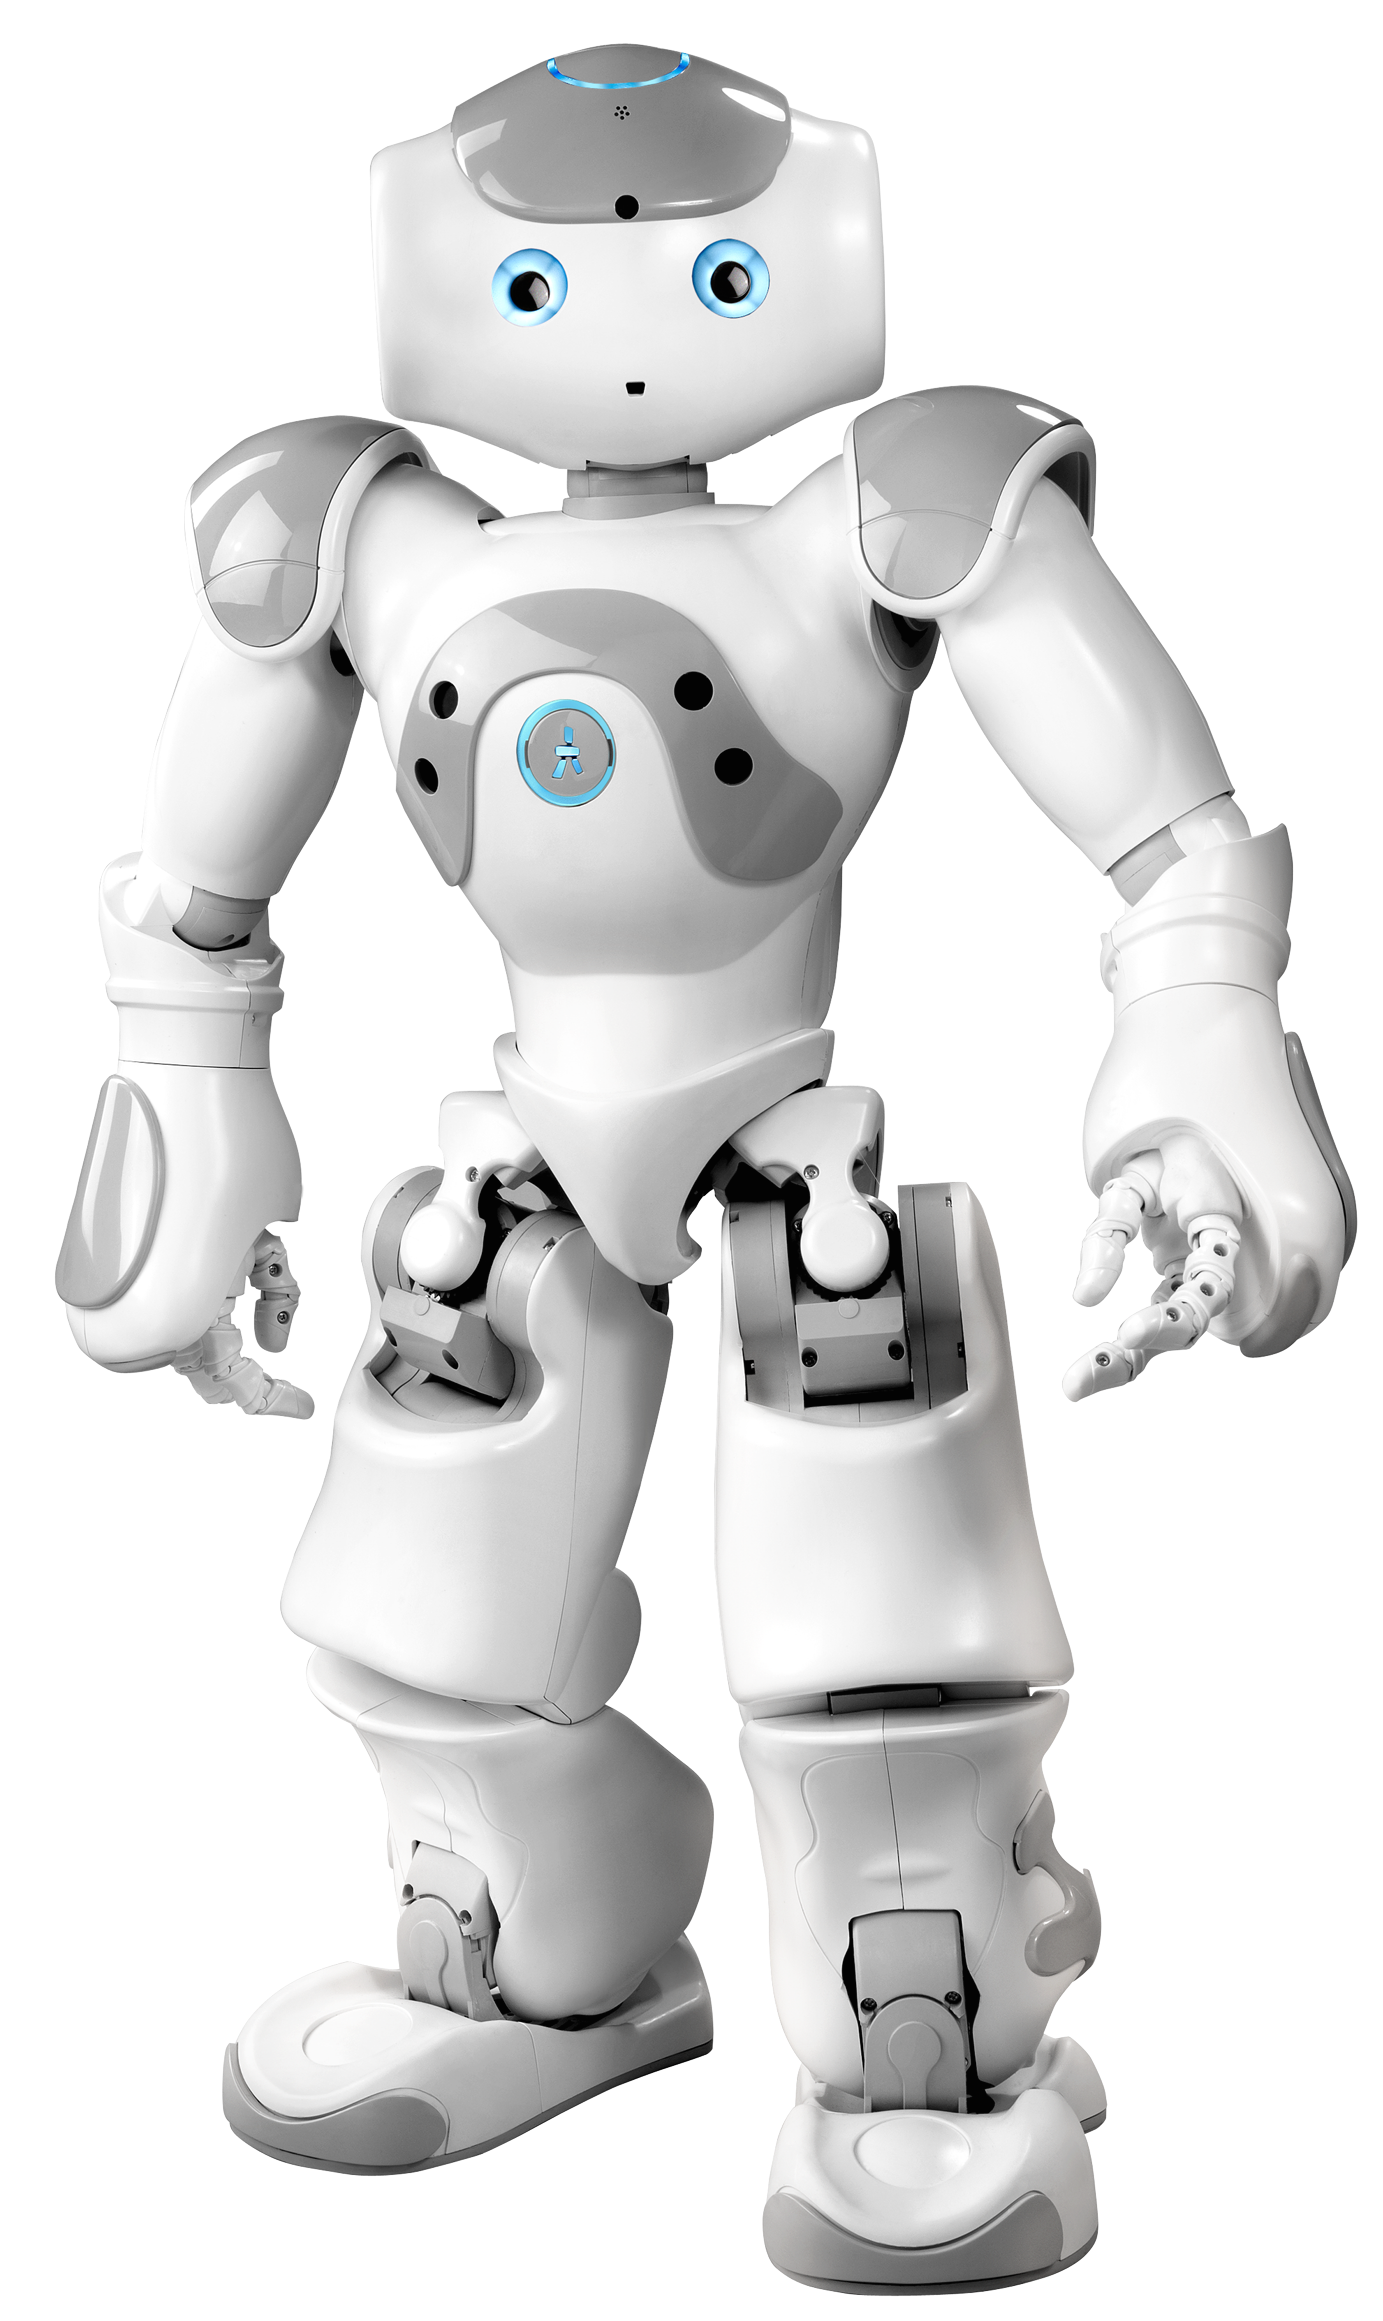
\includegraphics[height=5cm]{nao_face.png}}
    \hfil
    \subfloat[][Darwin-Op]{\label{fig:darwin_platform}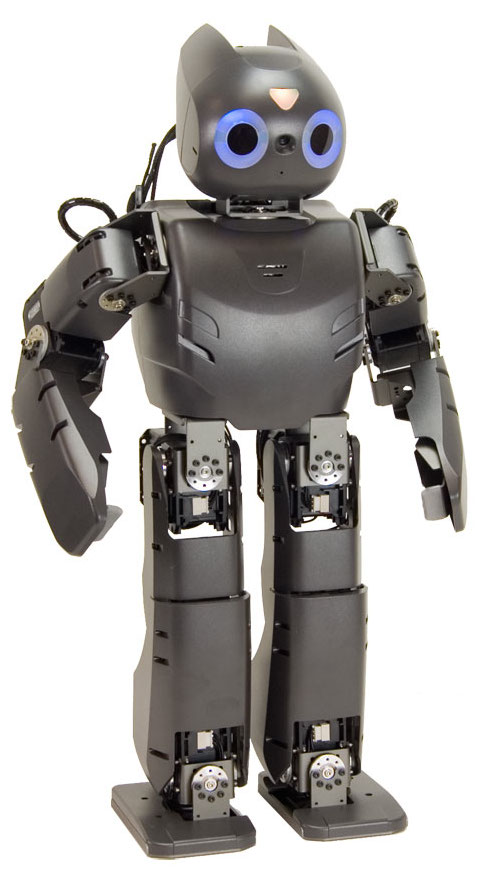
\includegraphics[height=5cm]{darwin_op_face.jpg}}
    \hfil
    \subfloat[][Acroban]{\label{fig:acroban_platform}\includegraphics[height=5cm]{acroban_wout_background.jpg}}
    \caption{None of the existing platforms in 2012 were suitable for exploring the role of morphology. Nao was impossible to modify. Darwin Op and Acroban used aluminium parts that are really difficult and expensive to produce.}
    \label{fig:2012_Humanoids}
\end{figure}

We also used Acroban (see \figurename~\ref{fig:acroban_platform}) designed by Olivier Ly~\cite{Ly2010}. It is a handcrafted humanoid platform created to explore certain morphological properties, especially compliance, with the aim of achieving dynamic locomotion and playful physical human robot interaction.
While it actually allows modification of its is morphology, it is manufactured from aluminium mechanical parts, Robotis Dynamixel motors, scotch, and rubber bands cobbled together, and changing it requires lot of effort . The manufacture of aluminium parts required is especially complicated and requires either very good handiwork or a 3-axis CNC.
In addition, its use was quite complicated and while several researchers could have been interested by Acroban to study human robot interaction and social acceptance, it was not possible to use it without getting our hands dirty.
Finally, the material and manufacturing process make the platform non-stationary. Even if a lab manages to reproduce it, there is a high probability that the physical properties will not be the same. Therefore, the diffusion and the reproducibility of results are limited.


A last alternative would be the use of Darwin Op robot (see \figurename~\ref{fig:darwin_platform}) which is both open source and easily accessible (Robotis sells it already assembled for \$10K), yet as Acroban its hardware consists of manufactured metal parts making its morphology very difficult and expensive to modify (see section REF for more details). Moreover, , even if Darwin is open source and very popular, to our knowledge its morphology has never be modified by the research community.

Thus one of the main goals was to successfully design a humanoid robot which can merge the advantages of both kind of robot, i.e. simple, accessible, reproducible and allowing to easily change and hack its morphology for scientific experiments that can be both customized and shared.

\subsection{An experiment-proof robot} % (fold)

Most researchers can attest to the difficulty and frustration faced while conducting robotic experimentation in the real world. We are challenged daily by bugs, technical issues, unpredicted events and side effects. While a bug in software can be fixed, an error with a hardware platform can cause damage to the robot and postpone the results of an experiment by several weeks.

Therefore many researchers in robotics avoid technical issues associated with the real world experimentation by using simple models and physical simulation. But the real world is extremely more complex and richer than the virtual one.
Some high-level behaviour experiments are conducted in simulators based on the hypothesis that real-world constraints are not relevant, yet it is really certain?
Indeed, while the real world constitutes a lot of constraints, it is also rich in complex physical effects (gravity, friction, inertia), which should be taken into consideration and could be very useful if interacting with the agent.

As we saw in the related work (chapter~\ref{REF}), the emergence of complex behaviours appears thanks to the interaction between the real world and simple robotic systems. We cannot program behaviour because behaviour is the result of interaction  between the program and the real world. Thus we cannot design behaviour without the ecological niche of the robot~\cite{Steels1991emergence}.

While using simulators can be helpful as a first step to design robots, it appears incomplete when showing results on the role of morphology without real world experimentation.
Therefore, when one wants to study the role of morphology on robot behavior, being able to explore it in the real world is of paramount importance. Unfortunately, current tools make the experimental step really hard to achieve for researchers.

Throughout our work on building cognitive and developmental learning algorithms, we have experienced these issues, especially while building and using Acroban~\cite{Ly2010} and during the Ergo robot experience (see section~\ref{REF}). Much time has been spent debugging non-robust technologies but it has been very instructive for understanding those that are efficient and those that should be avoided.
Therefore Poppy has been designed based on the background experience we have acquired building using robots acting in the real world.

\begin{description}
    \item[Robustness and Safety:] Demanding and lengthy real-world experimentation necessitates that the robot be robust and safe. It should be able to sustain experiments and fall down without easily breaking. At the same time, one should ensure that physical interaction with the robot is safe for humans.
    \item [Precision, stationary:]Experiments should be repeatable, implying that the robot properties should be stationary.
    \item [Breakable, repairable:] Breaking should not be costly and the robot should be easily repairable.
    \item [Transportable:] To allow for experiments in natural environments, possibly involving interaction with non-technical humans, the robot should be transportable outside the laboratory.
    \item [Easy and fast to duplicate:]If the robotic platform is to be reused  in this way, it must be easy and fast to duplicate.
    \item [Affordable:] To ensure widespread use, a key factor is to keep the cost of the platform relatively low. The more labs can be involved, the greater the scientific impact.
\end{description}



